% Phenotypic insufficiency of local protein representations: fibre-preserving rearrangements of human
% C2H2 zinc-finger arrays reorder DNA-recognition residues under an invariant 25-spectrum
% Build (in this folder): pdflatex zinc_finger_order (x2); figures are read from ../figures
\documentclass[11pt]{article}
\usepackage{lmodern}
\usepackage[T1]{fontenc}
\usepackage{amsmath,amssymb,amsthm,mathtools}
\usepackage[margin=1.05in]{geometry}
\usepackage{booktabs,array}
\usepackage{microtype}
\usepackage{graphicx}
\graphicspath{{../figures/}}
\usepackage{xcolor}
\usepackage{tikz}
\usetikzlibrary{arrows.meta,positioning}
\usepackage[hidelinks]{hyperref}
\newcommand{\doi}[1]{\href{https://doi.org/#1}{\nolinkurl{doi:#1}}}
\emergencystretch=2em

\theoremstyle{plain}
\newtheorem{theorem}{Theorem}
\newtheorem{proposition}[theorem]{Proposition}
\newtheorem{lemma}[theorem]{Lemma}
\newtheorem{corollary}[theorem]{Corollary}
\theoremstyle{definition}
\newtheorem{definition}[theorem]{Definition}
\theoremstyle{remark}
\newtheorem{remark}[theorem]{Remark}

\newcommand{\spec}{\operatorname{spec}}

\title{\bfseries Phenotypic insufficiency of local protein representations:\\
fibre-preserving rearrangements of human C2H2 zinc-finger arrays\\ reorder DNA-recognition residues under an
invariant 25-spectrum}
\author{Zhengyi Chen\\[2pt]
\normalsize\begin{tabular}{c}
Guangxi Key Laboratory of Drug Discovery and Optimization,\\
Guangxi Engineering Research Center for Pharmaceutical Molecular Screening\\
and Druggability Evaluation, School of Pharmacy, Guilin Medical University,\\
Guilin 541199, P.~R.~China\\
\texttt{chenzhengyi@glmc.edu.cn}
\end{tabular}
\and
Ruqing Chen\\[2pt]
\normalsize GUT Geoservice Inc., Montreal, Qu\'ebec, Canada\\
\normalsize\texttt{ruqing@hotmail.com}}
\date{25 September 2026}

\begin{document}
\maketitle

\begin{abstract}
\noindent
A protein representation that depends only on local sequence statistics assigns the same vector to all
sequences with the same multiset of $k$-mers, the \emph{spectral fibre}. Whether this matters depends on the
phenotype. For DNA-binding C2H2 zinc-finger proteins it does. Each finger reads about three base pairs through
residues at helix positions $-1$, $2$, $3$ and $6$, and the array reads its target in order. We show that for
$k$ at least the length of a finger, the \emph{multiset} of fingers is constant on the fibre, and only their
\emph{order} can change. We also give the exact condition for a reordering: the exchanged segments must be
bounded by repeated $(k-1)$-mers. The conserved TGEKP linker alone is far too short to bound one at $k=25$.
Among reviewed human proteins, $17$ C2H2 zinc-finger proteins have a non-trivial $25$-fibre. From $1\,178$
distinct fibre-mates drawn as random Eulerian trails, $883$ ($75\%$) place different recognition residues at
some array position. In ZNF91, a KRAB zinc-finger protein that represses SVA and L1 retrotransposons, one
fibre-mate changes the recognition residues at $17$ of $31$ array positions. In ZNF721 one changes $17$ of $23$.
Every window-$25$ local encoder is constant on these pairs, as verified for all $1\,178$. Under any
finger-additive recognition model, the predicted binding site differs exactly when the ordered recognition
residues differ. We formalize this as a phenotypic sufficiency criterion: a representation supports a
phenotype if and only if the phenotype is constant on its fibres. We then bound the error of every predictor
built on a local encoder. We did not measure binding. The predicted change of specificity rests on the additive
model, whose limits we discuss.
\end{abstract}

\medskip
\noindent\textbf{Keywords.} C2H2 zinc finger, KRAB zinc-finger proteins, DNA-binding specificity, recognition
code, spectral fibre, protein representation, sufficiency, ZNF91, ZNF721.

% ================================================================ 1
\section{Introduction}\label{sec:intro}

Protein sequence representations are often built from local statistics: amino acid and $k$-mer composition,
pseudo amino acid composition, and convolutional networks with global pooling. Such a representation is
constant on the \emph{spectral fibre} $F_k(S)$ of a sequence, the set of sequences with the same $k$-mer
multiset and the same first $(k-1)$-mer \cite{CC26a,CC26b,CC26d}. For $854$ reviewed human proteins the
$10$-mer spectrum does not determine the sequence. C2H2 zinc-finger proteins are $3.0\%$ of the proteome but
$40.7\%$ of those proteins \cite{CC26b}. Most of them are KRAB zinc-finger proteins (KZFPs).

That a representation is blind to a set of sequences does not by itself mean that it misses anything a
phenotype depends on. Most members of a fibre are not biologically meaningful \cite{CC26e}, and a phenotype
may be constant on the fibre. The question is therefore phenotype-specific. It needs a phenotype that is known
to depend on sequence order and not only on local content.

DNA recognition by tandem C2H2 zinc fingers is such a phenotype. Each finger contacts roughly three base pairs.
The fingers bind in antiparallel order, with the N-terminal finger at the $3'$ end of the site, and the site is
read as the ordered concatenation of the fingers' sub-sites \cite{PavletichPabo91,Wolfe00}. KZFPs, with arrays of
up to $30$ or more fingers, use this to recognize specific transposable-element families
\cite{Imbeault17,Jacobs14}. If a fibre-preserving rearrangement reorders the fingers, a local representation
cannot distinguish proteins that the recognition code says bind different sites.

This paper makes that argument exact and applies it to the human proteome. Section~\ref{sec:code} states the
recognition model and its limits. Section~\ref{sec:construction} proves that fibres preserve the multiset of
fingers and gives the condition under which they reorder it. Section~\ref{sec:cases} computes fibre-mates for
all $17$ human C2H2 zinc-finger proteins with a non-trivial $25$-fibre, with ZNF91 and ZNF721 as case studies.
Section~\ref{sec:sufficiency} formalizes phenotypic sufficiency and bounds what any predictor on a local
representation can achieve.

% ================================================================ 2
\section{The recognition code of tandem C2H2 zinc fingers}\label{sec:code}

A C2H2 zinc finger has the consensus $\mathtt C$-$X_{2\text{--}4}$-$\mathtt C$-$X_{12}$-$\mathtt H$-$X_{3\text{--}5}$-$\mathtt H$.
It folds into a $\beta\beta\alpha$ unit around a zinc ion. We number the recognition helix so that the first
zinc-coordinating histidine is at position $+7$; there is no position $0$. In the Zif268 structure, residues at
helix positions $-1$, $3$ and $6$ contact the $3'$, middle and $5'$ bases of a base triplet on the primary strand,
and position $2$ contacts the complementary strand \cite{PavletichPabo91,Elrod96}. Consecutive fingers occupy
consecutive triplets in antiparallel orientation, so the site of an array $f_1\cdots f_n$ reads, from $5'$ to $3'$,
\begin{equation}\label{eq:additive}
Y(S)=g(f_n)\,g(f_{n-1})\cdots g(f_1),
\end{equation}
where $g(f)$ is the sub-site (or the position-specific base preferences) of finger $f$. It depends on the
recognition residues $r(f)=(f_{-1},f_2,f_3,f_6)$ and, to a lesser degree, on other helix residues. We call a
recognition model \emph{finger-additive} if it has the form~\eqref{eq:additive} for some map $g$. Published
recognition codes predict $g$ from the helix residues, using structural rules, bacterial one-hybrid data or
machine learning \cite{PersikovSingh14,Najafabadi15}.

The additive model is an approximation. Neighbouring fingers influence each other through the position-2
contact and through the linker. Not all fingers of a long KZFP array engage DNA at once, and binding also depends
on chromatin \cite{Wolfe00,Imbeault17}. Our conclusions about binding are therefore conclusions about what the
additive model predicts. The conclusions about representations do not depend on it.

% ================================================================ 3
\section{Fibre-preserving rearrangements of finger arrays}\label{sec:construction}

Let $S\in\Sigma^L$ and $F_k(S)=\{T:\spec_k(T)=\spec_k(S),\ T[1..k-1]=S[1..k-1]\}$. All members of $F_k(S)$ also share the
last $(k-1)$-mer of $S$ \cite{CC26c}.

\begin{proposition}[the multiset of fingers is fibre-invariant]\label{prop:multiset}
For $T\in F_k(S)$ and every word $w$ with $|w|\le k$, $w$ occurs in $T$ as often as in $S$. In particular, if every
finger occurrence has length at most $k$, which holds for $k\ge24$ under the consensus above, $S$ and $T$ contain
the same multiset of fingers and the same multiset of recognition-residue tuples $r(f)$.
\end{proposition}

\begin{proof}
Every occurrence of $w$ starts at some position $p$. If $p\le L-k+1$, it is the prefix of exactly one $k$-mer
occurrence. Otherwise it lies in the last $(k-1)$-mer. Hence the number of occurrences of $w$ is the number of
$k$-mers in $\spec_k(S)$ with prefix $w$, plus the number of occurrences of $w$ in the last $(k-1)$-mer. Both are
the same for $T$. A finger occurrence spans $20$ to $24$ residues.
\end{proof}

So on a fibre of order $k\ge24$ a local representation cannot lose, gain or alter a finger. It can only fail to
see their arrangement. The arrangement changes by the elementary fibre moves: $S$ and $T$ in the same fibre differ
by a sequence of exchanges of two adjacent segments, each beginning and ending with an occurrence of the same
$(k-1)$-mer \cite{Ukk92,Pev95}.

\begin{proposition}[when fingers can change places]\label{prop:swap}
Let $S=A\,uXu\,Yu\,B$, where $u$ is a word of length $k-1$ and $X$, $Y$ are arbitrary. Then $T=A\,uYu\,Xu\,B$ lies in $F_k(S)$.
Conversely, every $T\in F_k(S)$ arises from $S$ by a finite sequence of such exchanges. In particular, two blocks of
fingers can exchange places only if they are bounded by a repeated word of length $k-1$. A linker motif of length
$\ell$ that is identical between fingers bounds such an exchange only for $k\le\ell+1$.
\end{proposition}

\begin{proof}
The first part is the standard transposition argument: the $k$-mers inside $uXu$ and $uYu$ are unchanged, and
the $k$-mers across each boundary read $u$ followed by the first letter of the next block, which is the same
multiset in $S$ and $T$ \cite{Ukk92}. The converse is the theorem of Ukkonen and Pevzner \cite{Ukk92,Pev95}. The
last statement follows because a boundary must be a repeated $(k-1)$-mer.
\end{proof}

The canonical KZFP linker \texttt{TGEKP} is $5$ residues long and bounds exchanges only for $k\le6$. At $k=25$ a
boundary must be a $24$-residue word that recurs, i.e.\ two stretches of the array that agree over most of a
finger. Such near-identity arises from recent duplication of fingers within an array, the process by which KZFP
arrays expand \cite{Imbeault17}.

\begin{figure}[t]
\centering
\resizebox{0.95\textwidth}{!}{%
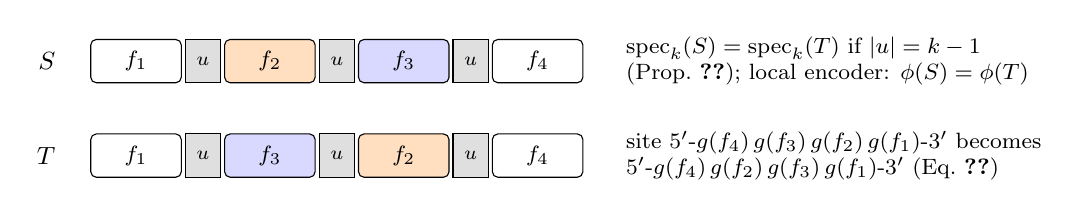
\begin{tikzpicture}[font=\small,
  f/.style={draw, rounded corners=2pt, minimum width=1.15cm, minimum height=0.55cm, font=\footnotesize},
  u/.style={draw, fill=gray!25, minimum width=0.45cm, minimum height=0.55cm, font=\scriptsize}]
\node[anchor=east] at (-0.3,1.2) {$S$};
\node[f] at (0.6,1.2) {$f_1$}; \node[u] at (1.45,1.2) {$u$};
\node[f, fill=orange!25] at (2.3,1.2) {$f_2$}; \node[u] at (3.15,1.2) {$u$};
\node[f, fill=blue!15] at (4.0,1.2) {$f_3$}; \node[u] at (4.85,1.2) {$u$};
\node[f] at (5.7,1.2) {$f_4$};
\node[anchor=east] at (-0.3,0) {$T$};
\node[f] at (0.6,0) {$f_1$}; \node[u] at (1.45,0) {$u$};
\node[f, fill=blue!15] at (2.3,0) {$f_3$}; \node[u] at (3.15,0) {$u$};
\node[f, fill=orange!25] at (4.0,0) {$f_2$}; \node[u] at (4.85,0) {$u$};
\node[f] at (5.7,0) {$f_4$};
\node[align=left, anchor=west, font=\footnotesize] at (6.7,1.2) {$\spec_k(S)=\spec_k(T)$ if $|u|=k-1$\\ (Prop.~\ref{prop:swap}); local encoder: $\phi(S)=\phi(T)$};
\node[align=left, anchor=west, font=\footnotesize] at (6.7,0) {site $5'\text{-}g(f_4)\,g(f_3)\,g(f_2)\,g(f_1)\text{-}3'$ becomes\\
  $5'\text{-}g(f_4)\,g(f_2)\,g(f_3)\,g(f_1)\text{-}3'$ (Eq.~\ref{eq:additive})};
\end{tikzpicture}}
\caption{A fibre-preserving exchange of fingers. When the blocks containing $f_2$ and $f_3$ are bounded by copies of
the same $(k-1)$-mer $u$ (grey), exchanging them preserves the $k$-spectrum, so every local encoder of order $k$ is
unchanged. Under a finger-additive recognition model the predicted site changes whenever $g(f_2)\ne g(f_3)$.}\label{fig:scheme}
\end{figure}

\begin{proposition}[additive models see the order]\label{prop:site}
Let $T\in F_k(S)$ with $k\ge24$, and let $r_1,\dots,r_n$ and $r'_1,\dots,r'_n$ be the recognition-residue tuples of the
finger arrays of $S$ and $T$ in array order. For every finger-additive model whose $g$ depends only on $r$,
$Y(S)=Y(T)$ whenever $r_i=r'_i$ for all $i$. If $g$ is injective on the tuples that occur, then $Y(S)\ne Y(T)$
whenever $r_i\ne r'_i$ for some $i$.
\end{proposition}

\begin{proof}
By Proposition~\ref{prop:multiset} both arrays have $n$ fingers, so $Y(S)$ and $Y(T)$ are concatenations of $n$
sub-sites of equal length, compared position by position.
\end{proof}

Injectivity of $g$ is an idealization. Different fingers can prefer the same triplet, so the numbers below are
upper bounds on the pairs for which a given code predicts different sites. They are exact counts of pairs
for which the recognition residues are ordered differently.

% ================================================================ 4
\section{Case studies: fibre-mates of human zinc-finger proteins}\label{sec:cases}

\paragraph{Method.} We took all reviewed human proteins annotated with C2H2-type zinc fingers and with
$N_{25}>1$ in \cite{CC26a}. There are $17$. For each, we drew $300$ random Eulerian trails of the de~Bruijn graph of
order $25$ starting at the protein's first $24$-mer, and kept the distinct sequences $T\ne S$. These draws are not
uniform on the fibre. They serve as witnesses, not as a sample. For every mate we verified
$\spec_{25}(T)=\spec_{25}(S)$, parsed the fingers of $S$ and $T$ with the consensus motif, checked that the finger
multisets agree (Proposition~\ref{prop:multiset}), compared the recognition residues position by position along the
array, and applied a randomly initialized convolutional encoder of window $25$ with mean pooling (float64).

\begin{table}[t]
\centering\small
\begin{tabular}{lrrrrrrr}
\toprule
protein & $L$ & $\kappa$ & $\log_2N_{25}$ & fingers & distinct mates & new order & max.\ positions\\
\midrule
KLF18 & 1052 & 54 & 12.3 & 3 & 285 & 0 & 0\\
ZNF208 & 1280 & 95 & 21.2 & 36 & 300 & 300 & 33\\
ZNF254 & 659 & 38 & 1.0 & 13 & 1 & 1 & 2\\
ZNF283 & 679 & 28 & 1.0 & 15 & 1 & 1 & 6\\
ZNF347 & 839 & 35 & 2.0 & 17 & 3 & 3 & 6\\
ZNF594 & 807 & 30 & 1.0 & 21 & 1 & 1 & 2\\
ZNF595 & 648 & 26 & 2.0 & 17 & 3 & 3 & 9\\
ZNF676 & 588 & 38 & 1.0 & 14 & 1 & 1 & 2\\
ZNF709 & 641 & 34 & 4.6 & 19 & 23 & 22 & 6\\
ZNF721 & 911 & 32 & 8.4 & 23 & 198 & 196 & 17\\
ZNF729 & 1252 & 42 & 9.8 & 34 & 246 & 245 & 23\\
ZNF761 & 746 & 27 & 2.0 & 17 & 3 & 3 & 11\\
ZNF840P & 716 & 33 & 1.0 & 18 & 1 & 1 & 2\\
ZNF888 & 718 & 26 & 1.0 & 17 & 1 & 1 & 2\\
ZNF91 & 1191 & 51 & 5.0 & 31 & 31 & 28 & 17\\
ZNF93 & 620 & 31 & 2.6 & 16 & 5 & 5 & 9\\
ZNF99 & 864 & 49 & 6.4 & 21 & 75 & 72 & 9\\
\midrule
total & & & & & 1\,178 & 883 & \\
\bottomrule
\end{tabular}
\caption{Fibre-mates of order $25$ of the $17$ human C2H2 zinc-finger proteins with $N_{25}>1$. ``New order'': mates in
which some array position carries different recognition residues $(-1,2,3,6)$. ``Max.\ positions'': the largest number
of such array positions in one mate. In all $1\,178$ mates the finger multiset equals that of $S$, and the window-$25$
encoder output is identical to that of $S$ (relative difference below $10^{-12}$).}\label{tab:proteins}
\end{table}

\paragraph{Results.} Table~\ref{tab:proteins} lists the proteins. Of $1\,178$ distinct fibre-mates, $883$ ($75\%$)
reorder the recognition residues. In every one of them the finger multiset is unchanged and the local encoder
output is identical. KLF18 is an instructive exception. Its fibre is large ($\log_2N_{25}=12.3$), but its repeats lie
outside its three fingers, so none of its $285$ mates reorders them. For the binding-site phenotype, a local encoder of
order $25$ loses nothing on KLF18.

\paragraph{ZNF91.} ZNF91 is a primate KZFP with $31$ fingers. It binds and represses SVA and L1 retrotransposons, and its
array expanded in the primate lineage \cite{Jacobs14}. Its $25$-fibre has $2^{5.0}$ members. In the mate shown in
Figure~\ref{fig:ladder}, fingers $3$--$19$ are rearranged. Two blocks of the array exchange places across a
$24$-residue boundary shared by near-identical fingers, and $17$ of the $31$ array positions carry different
recognition residues. Fingers $1$--$2$ and $20$--$31$ are unchanged. 

Under~\eqref{eq:additive}, the predicted $93$-bp binding site changes at $17$ of its $31$ triplets, while every local
encoder of order $25$ assigns the wild-type protein and its fibre-mate the exact same representation vector.

\paragraph{ZNF721.} ZNF721 has $23$ C2H2 fingers and $\log_2N_{25}=8.4$. Among the $198$ distinct fibre-mates drawn at
$k=25$, $196$ ($99\%$) reorder the recognition-residue tuples. In the mate shown in Figure~\ref{fig:ladder}b, an
internal block permutation across repeated $24$-mer boundaries alters the recognition tuples at $17$ of the $23$ array
positions, while preserving the finger multiset and all $25$-mer counts.

\begin{figure}[t]
\centering
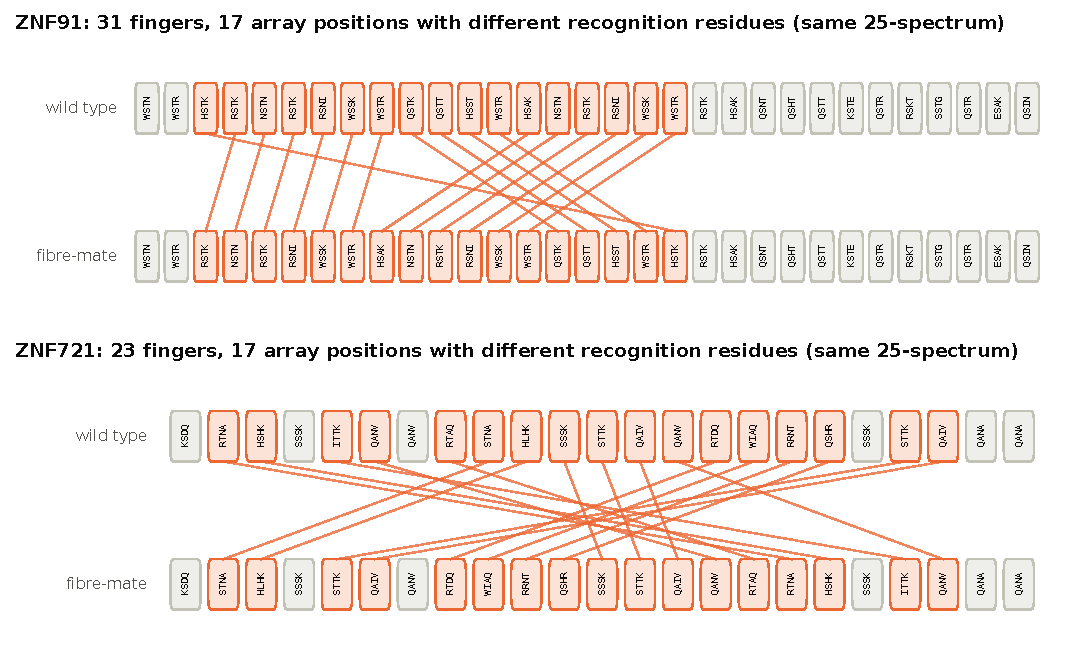
\includegraphics[width=\textwidth]{fig_ladder.pdf}
\caption{Fibre-preserving finger reorderings at $k=25$. Array positions of the C2H2 fingers in the wild-type protein
$S$ (top) and in a $25$-fibre mate $T\in F_{25}(S)$ (bottom) for (a)~ZNF91 ($31$ fingers; $17$ positions receive a
different recognition quartet) and (b)~ZNF721 ($23$ fingers; $17$ positions change). Slanted lines connect fingers
that move to a new array position; unmoved fingers are unmarked. In both cases $\spec_{25}(S)=\spec_{25}(T)$ and every
window-$25$ local encoder gives identical outputs on $S$ and $T$.}\label{fig:ladder}
\end{figure}

% ================================================================ 5
\section{Phenotypic sufficiency and predictor error bounds}\label{sec:sufficiency}

We now state the general condition under which an encoder's fibres force prediction errors on a downstream phenotype.
Let $\mathcal X\subseteq\Sigma^*$ be a domain of sequences, $\phi\colon\mathcal X\to\mathcal Z$ an encoder with fibres
$F_\phi(S)=\{T\in\mathcal X:\phi(T)=\phi(S)\}$, and $Y\colon\mathcal X\to\mathcal Y$ a phenotype map.

\begin{definition}[phenotypic sufficiency]\label{def:suff}
An encoder $\phi$ is \emph{phenotypically sufficient} for $Y$ on $\mathcal X$ if $Y$ is constant on every fibre of
$\phi$, i.e.\ $\phi(S)=\phi(T)$ implies $Y(S)=Y(T)$ for all $S,T\in\mathcal X$.
\end{definition}

\begin{theorem}[sufficiency criterion and irreducible error]\label{thm:bound}
Let $\phi\colon\mathcal X\to\mathcal Z$ and $Y\colon\mathcal X\to\mathcal Y$.
\begin{enumerate}
\item There exists a predictor $h\colon\mathcal Z\to\mathcal Y$ with $h(\phi(S))=Y(S)$ for all $S\in\mathcal X$ if and
only if $\phi$ is phenotypically sufficient for $Y$ on $\mathcal X$.
\item Let $d$ be a metric on $\mathcal Y$. For every pair $S,T\in\mathcal X$ in the same $\phi$-fibre and every
predictor $h\colon\mathcal Z\to\mathcal Y$,
\[
\max\bigl(d(h(\phi(S)),Y(S)),\;d(h(\phi(T)),Y(T))\bigr)\;\ge\;\frac12\,d(Y(S),Y(T)),
\]
and if $X$ is distributed uniformly on $\{S,T\}$, then $\mathbb E\,d(h(\phi(X)),Y(X))\ge\frac12\,d(Y(S),Y(T))$.
\end{enumerate}
\end{theorem}

\begin{proof}
(1) If $h\circ\phi=Y$, then $\phi(S)=\phi(T)$ implies $Y(S)=h(\phi(S))=h(\phi(T))=Y(T)$. Conversely, if $Y$ is
constant on every fibre, setting $h(z)=Y(S)$ for any $S\in\phi^{-1}(z)$ is well defined and satisfies $h(\phi(S))=Y(S)$.
(2) Since $\phi(S)=\phi(T)$, both predictions equal the same point $y=h(\phi(S))\in\mathcal Y$. By the triangle
inequality, $d(Y(S),Y(T))\le d(Y(S),y)+d(y,Y(T))$, so the sum of the two errors is at least $d(Y(S),Y(T))$ and their
maximum (and mean) is at least half of it.
\end{proof}

Combined with Proposition~\ref{prop:site} and Section~\ref{sec:cases}, Theorem~\ref{thm:bound} shows that on the
$25$-fibres of $16$ human C2H2 zinc-finger proteins, no local encoder of order $k\le25$ is phenotypically sufficient
for any injective finger-additive specificity model: every predictor built on $\phi$ incurs an error of at least half
the motif distance between $Y(S)$ and $Y(T)$ on each reordered fibre pair.

% ================================================================ 6
\section{Discussion and limitations}\label{sec:discussion}

The gap between separating a reference set and resolving a sequence becomes a phenotypic blind spot as soon as two
conditions meet: the protein's architecture places multiple domain copies between shared $(k-1)$-mer boundaries, and
the biological function depends on the order in which those copies sit. Tandem C2H2 zinc-finger arrays satisfy both.
At $k=25$, the fibre preserves the exact collection of fingers (Proposition~\ref{prop:multiset}) while permuting blocks
of fingers bounded by $24$-residue repeats (Proposition~\ref{prop:swap}). For $16$ human zinc-finger proteins,
including the retrotransposon repressors ZNF91 and ZNF93, such permutations reorder up to $17$--$33$ recognition
helices while leaving every order-$25$ local representation unchanged.

\paragraph{Limitations.} First, we did not measure DNA binding experimentally, nor did we run structural docking. The
claim that $Y(S)\ne Y(T)$ rests on the finger-additive recognition model~\eqref{eq:additive}. While the antiparallel
ordering of triplet contacts is established by co-crystal structures and ChIP-exo footprints
\cite{PavletichPabo91,Wolfe00,Imbeault17}, only a subset of fingers in a long KZFP array may contact DNA at a given
locus, so reordering non-contacting fingers would not alter binding at that locus. Second, the fibre-mates in
Section~\ref{sec:cases} are mathematical Eulerian trails of $G_{25}(S)$, not documented natural alleles; whether unequal
crossing-over or ectopic gene conversion produces these specific block permutations in human populations requires
long-read polymorphism data. Third, our theorems apply to local encoders. Protein language models with rotary or
relative positional encodings are not local \cite{CC26d}; whether their learned representations separate
finger-reordered mates is an empirical benchmark question.

\section*{Data and code availability}
The script \texttt{code/finger\_order.py} downloads the UniProt human proteome snapshot (or reads it from cache),
extracts C2H2 zinc fingers, draws fibre-mates at $k=25$, verifies $25$-spectrum and window-$25$ CNN invariance, and
writes \texttt{results/finger\_order.json}, \texttt{results/finger\_order\_output.txt} and
\texttt{results/finger\_pairs.tsv}, as well as \texttt{figures/fig\_ladder.pdf}. Code, results and figures are at
\url{https://github.com/Ruqing1963/zinc-finger-order}.

\section*{Funding}
This project was supported by the National Natural Science Foundation of China (No.~22464010), the
Guangxi Natural Science Foundation of China (No.~2025GXNSFAA069294), and the 2025 Bagui Youth Top
Talent Project.

\begin{thebibliography}{99}
\bibitem{CC26a} Z.~Chen, R.~Chen, \emph{What a local encoder cannot see: spectral fibres of the human proteome
and the representation of perturbagens}, Zenodo (2026). \doi{10.5281/zenodo.22950095}
\bibitem{CC26b} Z.~Chen, R.~Chen, \emph{Separation without resolution: the spectral fibre geometry of the human
proteome and the blind spots of local sequence encoders}, Zenodo (2026). \doi{10.5281/zenodo.22959211}
\bibitem{CC26c} Z.~Chen, R.~Chen, \emph{Information loss and quotient geometry of local sequence encoders:
representation lattices, fibre entropy and diameter bounds}, Zenodo (2026). \doi{10.5281/zenodo.22960439}
\bibitem{CC26d} Z.~Chen, R.~Chen, \emph{What finite-receptive-field encoders cannot distinguish: invariance
theorems and architectural boundaries of convolutional sequence models}, Zenodo (2026).
\doi{10.5281/zenodo.22963882}
\bibitem{CC26e} Z.~Chen, R.~Chen, \emph{Biologically reachable spectral fibres: repeat shuffling, copy ambiguity
and the scarcity of cryptic pathogenic missense variants in ClinVar}, Zenodo (2026).
\bibitem{Elrod96} M.~Elrod-Erickson, M.~A.~Rould, L.~Nekludova, C.~O.~Pabo, \emph{Zif268 protein--DNA complex
refined at 1.6~\AA: a model system for understanding zinc finger--DNA interactions}, Structure \textbf{4} (1996)
1171--1180. \doi{10.1016/S0969-2126(96)00125-6}
\bibitem{Imbeault17} M.~Imbeault, P.-Y.~Helleboid, D.~Trono, \emph{KRAB zinc-finger proteins contribute to the
evolution of gene regulatory networks}, Nature \textbf{543} (2017) 550--554. \doi{10.1038/nature21683}
\bibitem{Jacobs14} F.~M.~J.~Jacobs et al., \emph{An evolutionary arms race between KRAB zinc-finger genes ZNF91/93
and SVA/L1 retrotransposons}, Nature \textbf{516} (2014) 242--245. \doi{10.1038/nature13760}
\bibitem{Najafabadi15} H.~S.~Najafabadi et al., \emph{C2H2 zinc finger proteins greatly expand the human
regulatory lexicon}, Nat.\ Biotechnol.\ \textbf{33} (2015) 555--562. \doi{10.1038/nbt.3128}
\bibitem{PavletichPabo91} N.~P.~Pavletich, C.~O.~Pabo, \emph{Zinc finger--DNA recognition: crystal structure of a
Zif268--DNA complex at 2.1~\AA}, Science \textbf{252} (1991) 809--817. \doi{10.1126/science.2028256}
\bibitem{PersikovSingh14} A.~V.~Persikov, M.~Singh, \emph{De novo prediction of DNA-binding specificities for C2H2
zinc finger proteins}, Nucleic Acids Res.\ \textbf{42} (2014) 97--108. \doi{10.1093/nar/gkt890}
\bibitem{Pev95} P.~A.~Pevzner, \emph{DNA physical mapping and alternating Eulerian cycles in colored graphs},
Algorithmica \textbf{13} (1995) 77--105. \doi{10.1007/bf01188582}
\bibitem{Ukk92} E.~Ukkonen, \emph{Approximate string-matching with $q$-grams and maximal matches}, Theoret.\
Comput.\ Sci.\ \textbf{92} (1992) 191--211. \doi{10.1016/0304-3975(92)90143-4}
\bibitem{Wolfe00} S.~A.~Wolfe, L.~Nekludova, C.~O.~Pabo, \emph{DNA recognition by $\mathrm{Cys_2His_2}$ zinc finger
proteins}, Annu.\ Rev.\ Biophys.\ Biomol.\ Struct.\ \textbf{29} (2000) 183--212.
\doi{10.1146/annurev.biophys.29.1.183}
\end{thebibliography}

\end{document}